In this section, the terminology and concepts utilized throughout the paper are defined. The study is based on the Danish market for ancillary services, but the method presented here can be transferred to other markets.  

\subsection{Ancillary services}
Ancillary services are utilized by transmission system operators (TSOs) to ensure a adequate and secure operation of the power system. There is a variety of services targeting different aspects of the power system operation. This work will focus solely on active power control, but the method presented here can be translated into other types of services, e.g. control of reactive power for voltage control. Currently, frequency containment reserve (primary reserve) and frequency restoration reserve (secondary reserves) \cite{entso1operational} are widely utilized by TSOs to ensure frequency stability. In the future, such services are expected to be delivered by aggregators \cite{pudjianto2007virtual,vrettos2015frequency}. Furthermore, with the introduction of aggregators, new possibilities arise for solving problems at distribution system level, e.g. congestion issues, leading to new flexibility services being defined for distribution system operators (DSOs), as presented in \cite{ding2013development}. %, which can also be delivered by aggregators. This work will present an examle of each type of service.  
%defines seven DSO-flexibility services, which can be traded through a flexibility clearing house (FLECH). Five of these concern active power regulations and two voltage management services. 

\subsection{Flexible distributed energy resources}\label{sec:DERs}
With an increased electrification of the energy system due to the introduction of electric vehicles (EVs), heat pumps and local generation, DERs are expected to deliver an increasing amount of ancillary services in the future power grid. The DERs that can be utilized for ancillary services are those which can provide flexibility in consumption or generation without significantly impacting their primary energy service, e.g. battery state of charge and indoor temperature comfort \cite{costanzo2013coordination,halvgaard2012economic}.

The incentive for a DER owner of contracting an aggregator to manage his flexibility will likely be economical by receiving a payment for his availability. However, the incentive could also be non-economical; for example, the aggregator could offer actual services to the DER owner, e.g. efficient operation of heat pumps by live monitoring of the coefficient of performance or provision of a web interface for indoor climate control, which allows the DER owner to control the indoor temperature in his home. Another option could be that the aggregator controls a cluster of units owned by a single actor, e.g. the aggregator acts as a fleet operator for the optimal charging of a pool of EVs owned by single entity. Similarly, it could also be in control of the heating of an office building, where the overall temperature of all offices should respect certain comfort bounds. In the following, such services will be referred to as asset management services (AMS). % \bondynote{Anders, you had a few ideas here didn't you?}

%Examples of relevant DERs are electrical vehicles, which can charge dynamically and achieve peak-shaving at the point of connection, while still respecting some overall performance requirements like a specific state of charge in the morning \cite{costanzo2013coordination}. An electrical heat pump for residential heating can in some situations during winter shift its consumption more than half a day to achieve an economic benefit for the owner as described in \cite{halvgaard2012economic}. Residential refrigerators can significantly reduce the frequency nadir by providing a fast reacting primary reserve, while secondary reserves can come from electric water heaters and heating, ventilation and air conditioning systems of commercial buildings as described in \cite{vrettos2015frequency}.
%\subsection{Congestion management and DSO services}
%It is anticipated that the DSOs will start to utilize flexibility in the future (ref).
%
%Different grid tariffs are alternatives to power system services (NEAS ref).

\subsection{Players/roles in the market for ancillary services}
In Denmark, ancillary services are acquired by the TSO through an open market, where approved participants can bid their reserves. The bid size varies with the service, but generally the minimum bid size is larger than what most DERs can provide by themselves \cite{EnerginetAncillary}. Such market requirement further increases the need for aggregators, which can pool large amounts of DERs and represent them in the market as a single legal entity. Furthermore, most DER owners will likely not have the time, interest or knowledge to control their consumption 24 hours a day. 
%Because of this, a party called an Aggregator is needed, who pools a larger body of DER units and are responsible for the operation of these units. 
The aggregator can deliver TSO and DSO services as well as flexibility services for balance responsible parties (BRPs). BRPs are responsible for the balance of power production or consumption within their portfolio and they already trade energy in the power markets. The actors and their relationships can be seen in Fig.~\ref{fig:SEGANmarket}. Finally, in order to avoid the aggregator creating imbalances for the Balance Responsible Consumer, all aggregator-service sales must occur through the Balance Responsible Consumer. 
\begin{figure}
  \centering
  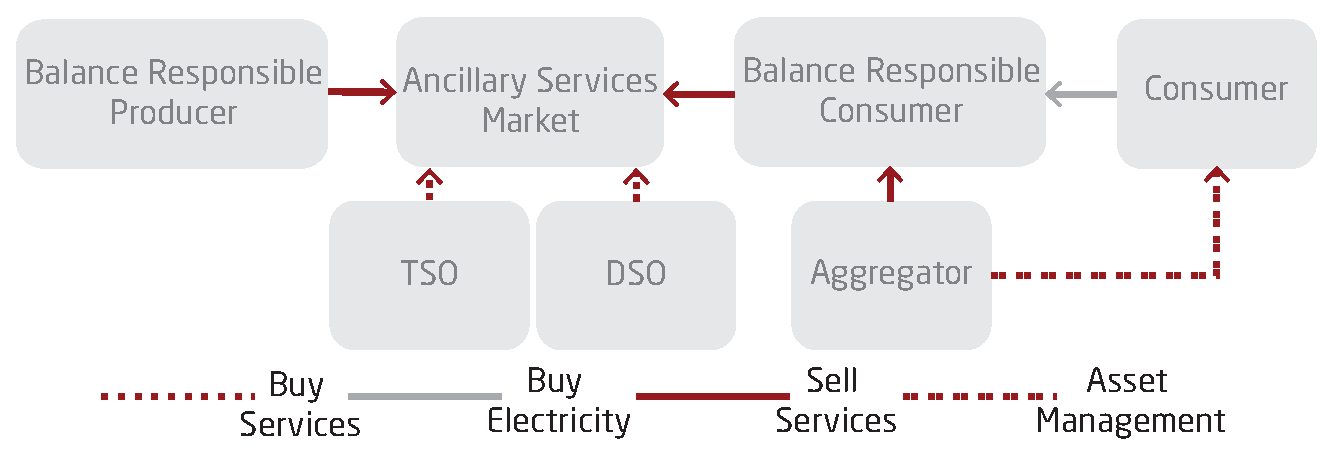
\includegraphics[width=\columnwidth]{SEGAN/market_future3.eps}
  \caption{The new player in the market for ancillary services is the aggregator, which sells consumption flexibility on the ancillary service markets through the Balance Responsible Consumer. Some markets allow the aggregators to participate directly in the ancillary service markets with the condition that they coordinate with their Balance Responsible Consumer.}
  \label{fig:SEGANmarket}
\end{figure}
%The aggregator will sign contracts with the DER owners and be the responsible party for delivery of service to the TSO, DSO or BRP. Further, the aggregator will have to ensure that certain performance parameters are respected towards the DER owner \cite{ding2013development}.
%Introduction of FLECH. \newline
